\begin{document}

NOTE: This text is about the model in examples/diffserv/simple_, which could be turned into a showcase.

\subsection{Simple domain example}


The \ffilename{examples/diffserv/simple\_} directory contains a
simple demonstration of Diffserv QoS capabilities.

\begin{center}
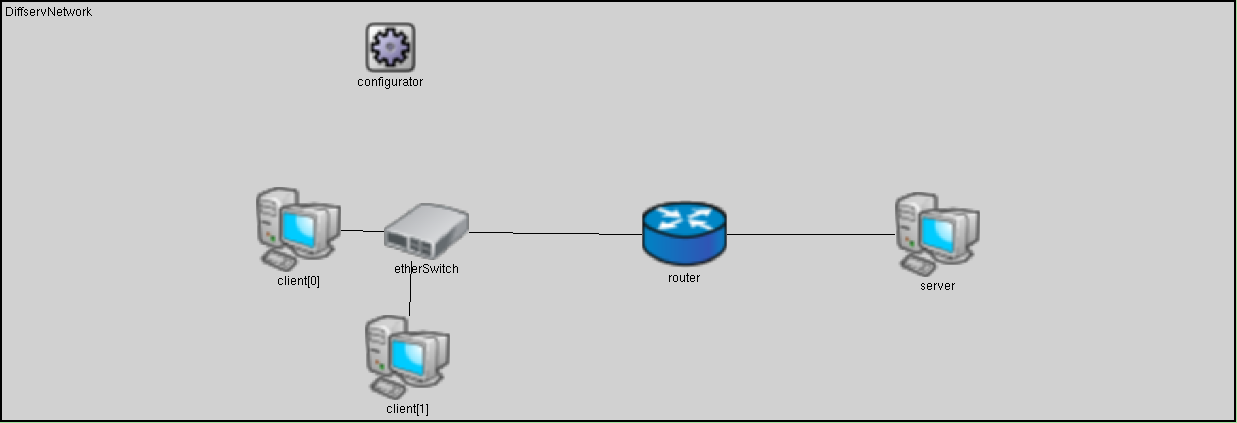
\includegraphics[scale=0.3]{figures/SimpleDiffservNetwork.png}
\end{center}

The network contains a router with an 10Mbps Ethernet interface and a
128kbps dialup link to a server. Clients are configured to generate
high traffic, that causes congestion at the router PPP interface.
One of the clients sends VoIP packets to the server.

With the \ttt{VoIP\_WithoutQoS} configuration, the queue in the router PPP interface
will be overloaded and packets are dropped randomly.

With the \ttt{VoIP\_WithPolicing} configuration, the VoIP traffic is classified as EF
traffic and the necessary bandwidth is allocated for it. The traffic conditioning
is configured so, that packets generated by the other clients are dropped if they
exceed the enabled rate.

With the \ttt{VoIP\_WithPolicingAndQueuing} configuration, the VoIP traffic is classified as EF
traffic and the necessary bandwidth is allocated for it. The router's queue is configured
so that EF packets are prioritized over other packets, so lower delays are expected.

After running these configuration you can see the statistics by opening the
VoIP.anf file, or can hear the difference by comparing the recorded .wav files
in the results directory.

\end{document}
